\documentclass[a4paper,12pt]{article}

%------------------------- packages -------------------------%
\usepackage[utf8]{inputenc}
\usepackage[T5]{fontenc}
\usepackage[vietnamese]{babel}
\usepackage[unicode,hidelinks]{hyperref}    % for reference
\usepackage{graphicx}
\usepackage{tikz}
\usepackage{amsmath}
\usepackage{geometry}
\usepackage{titlesec}
\usepackage{array}
\usepackage{fancyhdr}  % Ensure this is loaded last
\usepackage{lastpage}
\usepackage{setspace}
\usepackage{longtable}
\usetikzlibrary{calc}
\usepackage{tabularx}
\usepackage{array}  % For customizing row height
\usepackage{multirow} %dùng cho phần vẽ bảng ở phần lý thuyết
\usepackage[utf8]{inputenc}
\usepackage[utf8]{vietnam}
\usepackage{enumitem}
\usepackage{adjustbox}
\usepackage{amsmath,amsfonts,amssymb}
\usepackage{float}
\usepackage{array}
\usepackage{listings}
\usepackage{tcolorbox}
\usepackage{caption}
\usepackage{inconsolata}
\usepackage{listings}
\usepackage{tocloft} % for customizing TOC
\usepackage{indentfirst} % Bắt buộc đoạn đầu tiên sau tiêu đề phải thụt đầu dòng
\usepackage{subcaption}
\setlength{\parindent}{1.5em} % Thiết lập độ rộng thụt vào (có thể chỉnh thành 1cm, 2em...)

% for code and result
\lstset{
  breaklines=true,
  breakatwhitespace=true,
  basicstyle=\ttfamily\small, % Dùng font chữ nhỏ hơn
  columns=fullflexible
}

\lstdefinestyle{python}{
  language=Python,
  basicstyle=\ttfamily\footnotesize,
  keywordstyle=\color{blue!70!black}\bfseries,
  commentstyle=\color{green!40!black},
  stringstyle=\color{red!60!black},
%   numbers=left,
%   numberstyle=\tiny\color{gray},
%   numbersep=8pt,
  showstringspaces=false,
  breaklines=true,
  frame=single,
  rulecolor=\color{black!20},
  tabsize=4,
  backgroundcolor=\color{black!2},
}

\usepackage[svgnames]{xcolor} % Cung cấp nhiều màu sắc hơn
\tcbset{
  colback=AliceBlue,       % Màu nền xanh rất nhạt
  colframe=SteelBlue,      % Màu viền xanh dương đậm
  coltitle=MidnightBlue,   % Màu tiêu đề xanh đen
  coltext=DarkSlateGray,   % Màu chữ chính
  fonttitle=\bfseries      % Font chữ in đậm cho tiêu đề
}


%------------------------- set up -------------------------%
% Set the margins
\geometry{
    left=2cm,
    right=2cm,
    top=2.5cm,
    bottom=2.5cm,
}

%------------------------- header & footer -------------------------%
\renewcommand{\headrulewidth}{0.5pt}
\renewcommand{\footrulewidth}{0.5pt}
\setlength{\headheight}{30pt}
\pagestyle{fancy}

\fancyhead{}    % clear all header fields
\fancyhead[L]{
    \begin{tabular}{ll}
        \begin{picture}(10,10)
            \put(0,-7){
\includegraphics[width=8mm]{hcmut.png}}
        \end{picture}&
        \begin{tabular}{l}
            {\ttfamily Trường Đại học Bách Khoa Tp. Hồ Chí Minh} \\
            {\ttfamily Khoa Khoa học và Kỹ thuật Máy tính} \\
        \end{tabular} 	
    \end{tabular}
}

\fancyfoot{}    % clear all footer fields

\fancyfoot[R]{\footnotesize {\ttfamily Trang {\thepage}/\pageref{LastPage}}}

%------------------------- title format settings -------------------------%
\titleformat{\chapter}[display]
  {\normalfont\huge\bfseries}{\chaptertitlename\ \thechapter}{20pt}{\Huge}

% Multi-layered Blue Border Definition
\newcommand{\coverpageborder}{
    \begin{tikzpicture}[remember picture,overlay,inner sep=0,outer sep=0]
        \draw[blue!70!black,line width=4pt] 
            ([xshift=-1.5cm,yshift=-2cm]current page.north east) coordinate (A)--([xshift=1.5cm,yshift=-2cm]current page.north west) coordinate(B)--([xshift=1.5cm,yshift=2cm]current page.south west) coordinate (C)--([xshift=-1.5cm,yshift=2cm]current page.south east) coordinate(D)--cycle;
        \draw ([yshift=0.5cm,xshift=-0.5cm]A)-- ([yshift=0.5cm,xshift=0.5cm]B)--
        ([yshift=-0.5cm,xshift=0.5cm]B) --([yshift=-0.5cm,xshift=-0.5cm]B)--([yshift=0.5cm,xshift=-0.5cm]C)--([yshift=0.5cm,xshift=0.5cm]C)--([yshift=-0.5cm,xshift=0.5cm]C)-- ([yshift=-0.5cm,xshift=-0.5cm]D)--([yshift=0.5cm,xshift=-0.5cm]D)--([yshift=0.5cm,xshift=0.5cm]D)--([yshift=-0.5cm,xshift=0.5cm]A)--([yshift=-0.5cm,xshift=-0.5cm]A)--([yshift=0.5cm,xshift=-0.5cm]A);
        \draw ([yshift=-0.3cm,xshift=0.3cm]A)-- ([yshift=-0.3cm,xshift=-0.3cm]B)--
        ([yshift=0.3cm,xshift=-0.3cm]B) --([yshift=0.3cm,xshift=0.3cm]B)--([yshift=-0.3cm,xshift=0.3cm]C)--([yshift=-0.3cm,xshift=-0.3cm]C)--([yshift=0.3cm,xshift=-0.3cm]C)-- ([yshift=0.3cm,xshift=0.3cm]D)--([yshift=-0.3cm,xshift=0.3cm]D)--([yshift=-0.3cm,xshift=-0.3cm]D)--([yshift=0.3cm,xshift=-0.3cm]A)--([yshift=0.3cm,xshift=0.3cm]A)--([yshift=-0.3cm,xshift=0.3cm]A);
    \end{tikzpicture}
}

%------------------------- tocloft settings -------------------------%
\renewcommand{\listfigurename}{DANH MỤC HÌNH ẢNH}


\setlength{\cftbeforesecskip}{0pt} % Space before each section entry
\setlength{\cftsecnumwidth}{2em}   % Width of the section number
\setlength{\cftsubsecindent}{3em}  % Indentation for subsections
\setlength{\cftsubsecnumwidth}{3em}% Width of the subsection number
\setlength{\cftsubsubsecindent}{5em} % Indentation for subsubsections
\setlength{\cftsubsubsecnumwidth}{4em} % Width of the subsubsection number

%------------------------- body -------------------------%
\begin{document}

%-------------------- cover --------------------%
\begin{titlepage}
    \centering
    
    % Draw the cover page border
    \coverpageborder
    
    % University and Department Info
    \textbf{\large{ĐẠI HỌC QUỐC GIA THÀNH PHỐ HỒ CHÍ MINH}}\\[0.1cm]
    \textbf{\large{TRƯỜNG ĐẠI HỌC BÁCH KHOA}}\\[0.1cm]
    \textbf{\large{KHOA KHOA HỌC VÀ KỸ THUẬT MÁY TÍNH}}\\[0.25cm]
    
    % Logo Positioning
    
\includegraphics[width=0.5\textwidth]{hcmut.png}\\[0.3cm]
    
    % Title and Subtitle
    \textbf{\LARGE{BÁO CÁO HỌC PHẦN MỞ RỘNG}}\\[0.2cm]
    \textbf{\Large{CÔNG NGHỆ PHẦN MỀM (CO300A)}}\\[0.6cm]
    
    % Group Info
    \textbf{\large{Lớp: A01 - Nhóm 1}}\\[0.2cm]
    \textbf{\large{GVHD: Nguyễn Thành Công}}\\[0.2cm]
    \begin{table}[h]
    \renewcommand{\arraystretch}{1.5}  % Điều chỉnh chiều cao hàng (1.5 lần bình thường)
    \centering
    \begin{adjustbox}{max width=\textwidth} % Đảm bảo bảng vừa với chiều rộng trang
    \begin{tabular}{|c|l|c|c|c|}
        \hline
        \textbf{STT} & \multicolumn{1}{c|}{\textbf{Họ và tên}} & \textbf{MSSV} & \textbf{Tên lớp} & \textbf{Tên ngành} \\ \hline
        1 & Nguyễn Văn Hùng & 2311301 & A01 & Kỹ thuật máy tính \\ \hline
        2 & Trần Minh Trí & 2313626 & A01 & Kỹ thuật máy tính \\ \hline
        3 & Nguyễn Tô Quốc Việt & 2313898 & A01 & Kỹ thuật máy tính \\ \hline
        4 & Lê Công Vinh & 2313912 & A01 & Kỹ thuật máy tính \\ \hline
    \end{tabular}
    \end{adjustbox}
\end{table}
    
    \vspace{1.5cm} % Adjust space between the table and the advisor section
   
    
    % Date
    \textbf{\large{THÀNH PHỐ HỒ CHÍ MINH, THÁNG 4 NĂM 2026}}
\end{titlepage}


%------------------------- re-apply fancy page style -------------------------%
\pagestyle{fancy}

%------------------------- sections -------------------------%


\newpage
\setstretch{1.25}
\renewcommand{\baselinestretch}{1.25}

%=================== BODY CONTENT ===================%

\newpage
    {\large \textbf{BẢNG PHÂN CHIA CÔNG VIỆC}} \\[1.5ex] 
\begin{table}[h]
    \centering
    % Dòng chữ to chỉ định tên bảng

    
    \renewcommand{\arraystretch}{2.0}  % Điều chỉnh chiều cao hàng (tăng lên 2.0 để cao hơn)
    \begin{adjustbox}{max width=\textwidth} % Đảm bảo bảng vừa với chiều rộng trang
    \begin{tabular}{|c|l|c|c|c|}
        \hline
        \textbf{STT} & \multicolumn{1}{c|}{\textbf{Họ và tên}} & \textbf{MSSV} & \textbf{Đóng góp} & \textbf{Công việc cá nhân} \\ \hline
        1 & Nguyễn Văn Hùng & 2311301 & 100\% &  Implementation and Code Quality và Software Testing and Quality Assurance  \\ \hline
        2 & Trần Minh Trí & 2313626 & 100\% & Process Model and Planning và Architecture Design\\ \hline
        3 & Nguyễn Tô Quốc Việt & 2313898 & 100\% & Software Testing and Quality Assurance và Reflection and Retrospective \\ \hline
        4 & Lê Công Vinh & 2313912 & 100\% &  Requirements Engineering và System Modeling\\ \hline
    \end{tabular}
    \end{adjustbox}
\end{table}
    

\newpage
\setstretch{1.25}
\tocloftpagestyle{fancy}
\tableofcontents


\newpage


\cleardoublepage
\addcontentsline{toc}{section}{\listfigurename} % Đưa danh mục hình ảnh vào mục lục
\listoffigures
\newpage


% --- SECTION 1: INTRODUCTION ---
%Mục 1
\section{Requirements Engineering}

\textbf{Mục tiêu:} Xác định các chức năng của hệ thống và những đối tượng sẽ tương tác với hệ thống Smart Event Reminder System (SERS).

\subsection{Stakeholders}
Hệ thống bao gồm các bên liên quan chính sau đây:

\begin{table}[h]
\centering
\renewcommand{\arraystretch}{1.5}
\begin{tabular}{|p{4cm}|p{10cm}|}
\hline
\textbf{Stakeholder} & \textbf{Vai trò} \\ \hline
User & Tạo và quản lý các sự kiện cá nhân. \\ \hline
Admin & Quản lý tài khoản người dùng và giám sát dữ liệu hệ thống. \\ \hline
Notification Service & Thành phần kỹ thuật chịu trách nhiệm kích hoạt và gửi nhắc nhở. \\ \hline
Project Team & Nhóm sinh viên chịu trách nhiệm thiết kế, lập trình và kiểm thử. \\ \hline
Instructor & Giảng viên đánh giá quy trình và chất lượng tài liệu kỹ thuật. \\ \hline
\end{tabular}
\caption{Danh sách các bên liên quan của dự án SERS}
\end{table}

\subsection{Yêu cầu hệ thống}

\subsubsection{Functional Requirements - FR}
\begin{enumerate}
    \item \textbf{FR1:} Hệ thống cho phép người dùng tạo sự kiện mới.
    \item \textbf{FR2:} Hệ thống cho phép người dùng nhập chi tiết sự kiện (tiêu đề, mô tả, ngày, giờ, địa điểm).
    \item \textbf{FR3:} Hệ thống cung cấp chức năng chỉnh sửa thông tin các sự kiện đã tồn tại.
    \item \textbf{FR4:} Hệ thống cho phép người dùng xóa các sự kiện khỏi danh sách quản lý.
    \item \textbf{FR5:} Hệ thống tự động gửi nhắc nhở trước khi sự kiện bắt đầu theo thời gian đã cài đặt.
    \item \textbf{FR6:} Hệ thống hiển thị thông báo nhắc nhở khi người dùng nhập sau thông tin khi tạo sự kiện.
\end{enumerate}

\subsubsection{Non-Functional Requirements - NFR}
\begin{enumerate}
    \item \textbf{NFR1 (Hiệu năng):} Thông báo nhắc nhở phải được gửi đến người dùng trong vòng tối đa 60 giây kể từ thời điểm kích hoạt.
    \item \textbf{NFR2 (Tính khả dụng):} Giao diện người dùng phải trực quan, cho phép tạo một sự kiện trong ít hơn 3 phút thao tác.
    \item \textbf{NFR3 (Độ tin cậy):} Dữ liệu sự kiện phải được lưu trữ an toàn và không bị mất khi ứng dụng khởi động lại hoặc mất kết nối mạng tạm thời.
\end{enumerate}

\subsection{User Stories và Tiêu chí chấp nhận}

\begin{longtable}{|p{1cm}|p{6cm}|p{7cm}|}
\hline
\textbf{ID} & \textbf{User Story} & \textbf{Acceptance Criteria} \\ \hline
US1 & As a User, I want to create an event with a title, date, and time so that I can schedule my plans. & 1. Hệ thống lưu sự kiện khi điền đủ thông tin bắt buộc. \newline 2. Hiển thị thông báo lỗi nếu bỏ trống tiêu đề. \\ \hline
US2 & As a User, I want to edit event details so that I can update my schedule if plans change. & 1. Thông tin mới được cập nhật ngay lập tức vào cơ sở dữ liệu. \newline 2. Người dùng có thể hủy chỉnh sửa mà không mất dữ liệu cũ. \\ \hline
US3 & As a User, I want to delete an event so that I can remove cancelled activities. & 1. Yêu cầu xác nhận trước khi xóa. \newline 2. Sự kiện biến mất khỏi danh sách sau khi xóa thành công. \\ \hline
US4 & As a User, I want to receive a reminder so that I am not late for my events. & 1. Thông báo xuất hiện đúng thời gian quy định. \newline 2. Nội dung thông báo hiển thị đúng tiêu đề sự kiện. \\ \hline
US5 & As a User, I want to receive error notifications when entering invalid data so that I can ensure the event list remains accurate. & 1. Hệ thống hiển thị thông báo lỗi cụ thể khi người dùng nhập sai định dạng dữ liệu. \newline 2. Ngăn chặn việc lưu sự kiện vào danh sách nếu có trường dữ liệu không hợp lệ. \\ \hline
\end{longtable}

\subsection{Ưu tiên yêu cầu theo mô hình MoSCoW}

\begin{table}[H]
\centering
\renewcommand{\arraystretch}{1.3}
\begin{tabular}{|l|p{10cm}|}
\hline
\textbf{Phân loại} & \textbf{Tính năng / Yêu cầu} \\ \hline
\textbf{Must have} & Tạo, sửa, xóa sự kiện; Chức năng gửi nhắc nhở tự động. \\ \hline
\textbf{Should have} & Nhập chi tiết địa điểm; Xem danh sách sự kiện theo lịch. \\ \hline
\textbf{Could have} & Mời người dùng khác; Chia sẻ sự kiện qua mạng xã hội. \\ \hline
\textbf{Won't have} & Đồng bộ hóa với Google Calendar/Outlook (trong phiên bản này). \\ \hline
\end{tabular}
\caption{Bảng phân loại mức độ ưu tiên MoSCoW}
\end{table}

\subsection{Traceability Table}

\begin{table}[H]
\centering
\renewcommand{\arraystretch}{1.3}
\begin{tabular}{|c|c|p{9.5cm}|}
\hline
\textbf{Mã FR} & \textbf{Mã User Story} & \textbf{Biểu đồ liên quan} \\ \hline
FR1, FR2 & US1 & Sequence Diagram (Create Event), Class Diagram, State Diagram\\ \hline
FR3, FR4 & US2 & Sequence Diagram (Edit/Deltete Event), Class Diagram, State Diagram \\ \hline
FR5 & US4 & State Diagram, Class Diagram \\ \hline
FR6 & US5 & Class Diagram \\ \hline
\end{tabular}
\caption{Traceability Table thể hiển liên kết giữa Yêu cầu, User Story và Diagram}
\end{table}

%Mục 2
\section{Process Model and Planning}
\subsection{Lựa chọn mô hình phát triển}
\begin{itemize}[leftmargin=*]
    \item \textbf{Mô hình được chọn:} Scrum (Agile).
    \item \textbf{Lý do nhóm chọn mô hình này:} 
    \begin{itemize}
        \item \textit{Phù hợp với tính chất dự án:} SERS yêu cầu phát triển nhanh các tính năng cốt lõi (tạo, sửa, xóa sự kiện) và có thể linh hoạt mở rộng. Việc áp dụng Scrum với các Sprint ngắn (2 tuần) giúp nhóm làm việc tập trung và dễ dàng đối phó với những thay đổi về thiết kế (ví dụ: cập nhật thêm class \texttt{NotificationService} hay \texttt{Reminder}).
        \item \textit{Tối ưu hóa nguồn lực nhóm 4 người:} Quy trình Scrum phân chia task minh bạch, giúp 4 thành viên dễ dàng phối hợp giữa việc vẽ Diagram, lập trình logic và kiểm thử (Testing) mà không bị chồng chéo công việc.
    \end{itemize}
\end{itemize}

\subsection{Quản lý Backlog và Ước lượng thời gian}
Nhóm sử dụng kỹ thuật \textbf{Planning Poker} để đánh giá độ phức tạp của từng User Story (US).

\subsubsection*{Product Backlog (Đồng bộ với MoSCoW)}
\begin{table}[hbt!]
    \centering
    \renewcommand{\arraystretch}{1.3}
    \begin{tabularx}{\textwidth}{|c|X|c|c|c|}
        \hline
        \textbf{ID} & \textbf{Hạng mục (User Story)} & \textbf{Độ ưu tiên} & \textbf{Story Points} & \textbf{Trạng thái} \\ \hline
        US1 & Tạo sự kiện mới với các thông tin (tiêu đề, ngày, giờ). & Must have & 5 & Sprint 1 \\ \hline
        US2 & Chỉnh sửa và cập nhật chi tiết sự kiện đã có. & Must have & 8 & Sprint 1 \\ \hline
        US3 & Xóa sự kiện khỏi danh sách. & Must have & 3 & Sprint 1 \\ \hline
        US4 & Hệ thống tự động gửi thông báo nhắc nhở. & Must have & 13 & Sprint 2 \\ \hline
        US5 & Mời người dùng khác tham gia sự kiện. & Could have & 8 & Backlog \\ \hline
        US6 & Xem danh sách sự kiện theo lịch trình. & Should have & 5 & Backlog \\ \hline
    \end{tabularx}
    \caption{Danh sách Product Backlog tổng thể}
\end{table}

\subsubsection*{Sprint Backlog (Sprint 1 - Kéo dài 2 tuần)}
\textbf{Mục tiêu Sprint:} Hoàn thiện logic nền tảng (CRUD) và vòng đời của sự kiện.
Để giám sát chặt chẽ, nhóm phân rã công việc bám sát vào các Diagram đã thiết kế:
\begin{itemize}[leftmargin=*]
    \item \textbf{Task 1.1 [US1, US2]:} Hiện thực cấu trúc dữ liệu cho các class \texttt{User}, \texttt{Event}, \texttt{Reminder} dựa trên \textbf{Class Diagram (Hình 4)}. (\textit{3 SP})
    \item \textbf{Task 1.2 [US1]:} Xây dựng luồng xử lý tạo sự kiện mới, bao gồm logic kiểm tra tính hợp lệ dữ liệu theo \textbf{Sequence Diagram (Hình 1)}. (\textit{5 SP})
    \item \textbf{Task 1.3 [US2, US3]:} Hiện thực chức năng chỉnh sửa và xóa sự kiện theo \textbf{Sequence Diagram (Hình 2)}. (\textit{5 SP})
    \item \textbf{Task 1.4 [US1, US2]:} Quản lý chuyển đổi trạng thái của Event (Draft $\rightarrow$ Scheduled $\rightarrow$ Editing...) bám sát \textbf{State Diagram (Hình 3)}. (\textit{1 SP})
    \item \textbf{Task 1.5 [US1, US3]:} Viết Unit Test và refactor mã nguồn. (\textit{2 SP})
\end{itemize}

\subsection{Theo dõi tiến độ}
\begin{table}[H]
    \centering
    \renewcommand{\arraystretch}{1.2}
    \begin{tabular}{|l|c|c|p{7.5cm}|}
        \hline
        \textbf{Thời gian} & \textbf{SP Dự kiến} & \textbf{SP Thực tế} & \textbf{Ghi chú tiến độ} \\ \hline
        Ngày 1 & 16 & 16 & Họp Sprint Planning, phân rã task theo UML. \\ \hline
        Ngày 4 & 13 & 13 & Hoàn thành Task 1.1 (Khởi tạo các Class lõi). \\ \hline
        Ngày 8 & 8 & 8 & Xong Task 1.2 (Pass luồng tạo Event - Hình 1). \\ \hline
        Ngày 12 & 3 & 3 & Xong Task 1.3 \& 1.4 (Sửa/Xóa Event \& Cập nhật State). \\ \hline
        Ngày 14 & 0 & 0 & Hoàn thành Unit Test (Task 1.5). Kết thúc Sprint 1. \\ \hline
    \end{tabular}
    \caption{Tiến độ thực hiện Sprint 1}
\end{table}
%Mục 3
\section{System Modeling}


\begin{figure}[H]
    \centering
    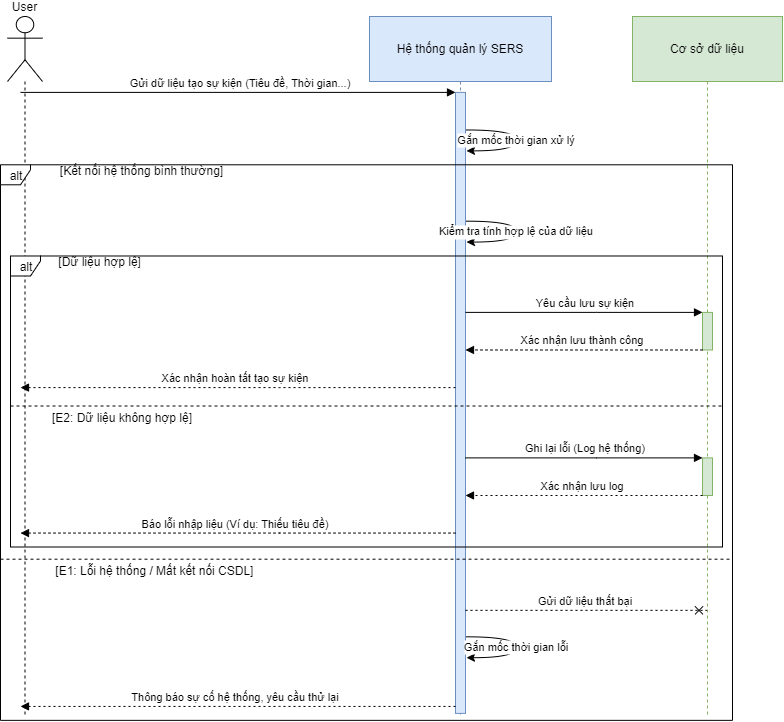
\includegraphics[width=0.7\textwidth]{pictures/seq1.png}
    \caption{Sequence Diagram mô tả cho việc tạo mới event}
\end{figure}

\begin{figure}[H]
    \centering
    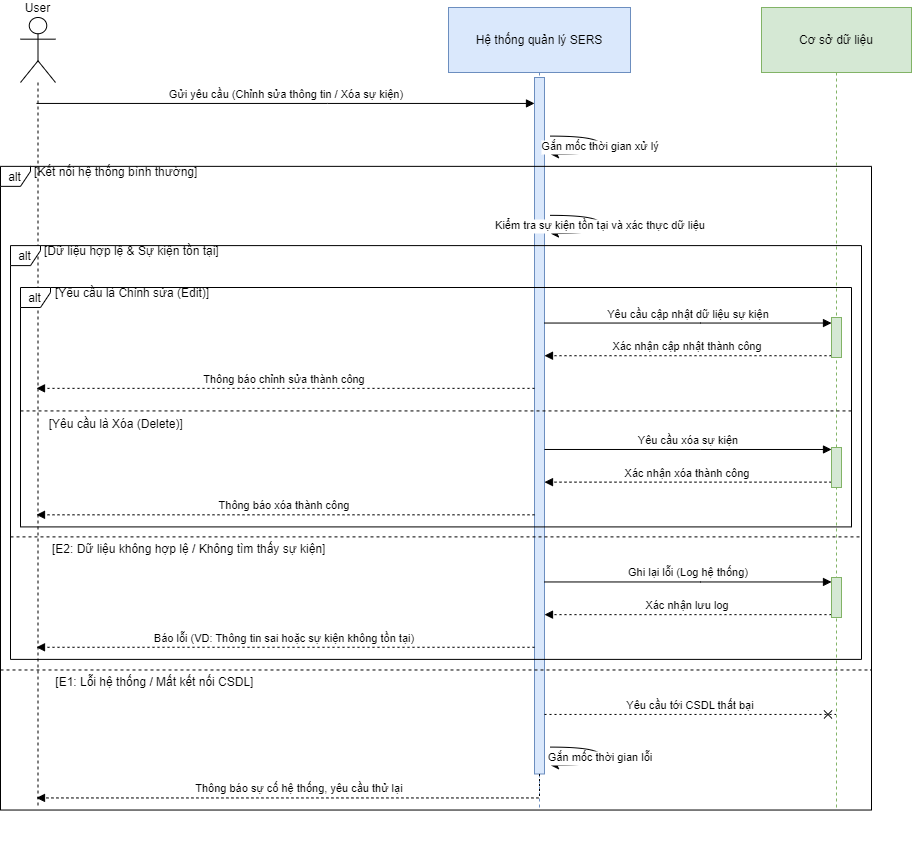
\includegraphics[width=0.7\textwidth]{pictures/seq2.png}
    \caption{Sequence Diagram mô tả cho việc chỉnh sửa và xóa event}
\end{figure}

\begin{figure}[H]
    \centering
    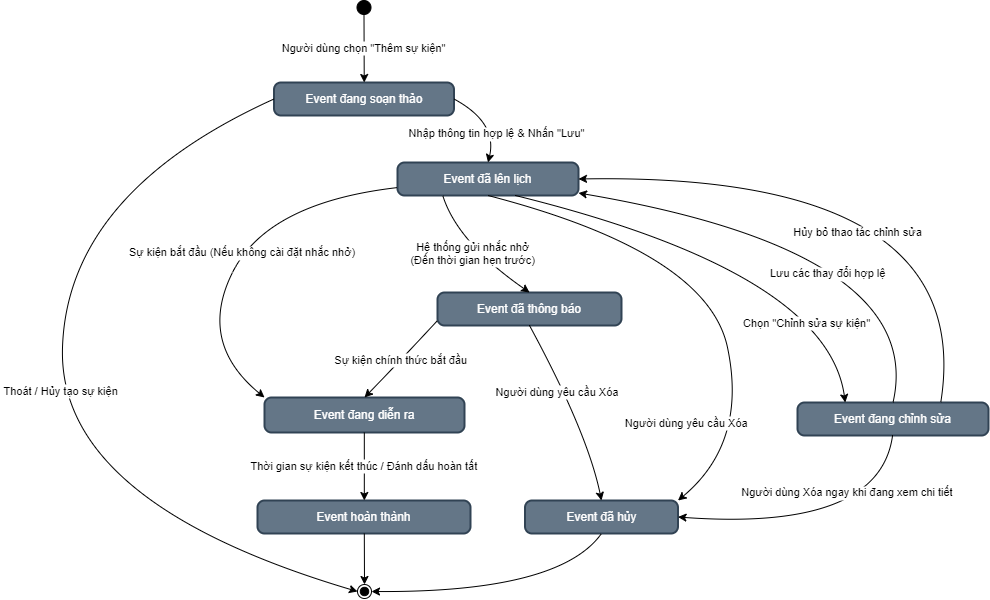
\includegraphics[width=1\textwidth]{pictures/statedia.png}
    \caption{State Diagram mô tả vòng đời các event}
\end{figure}

\begin{figure}[H]
    \centering
    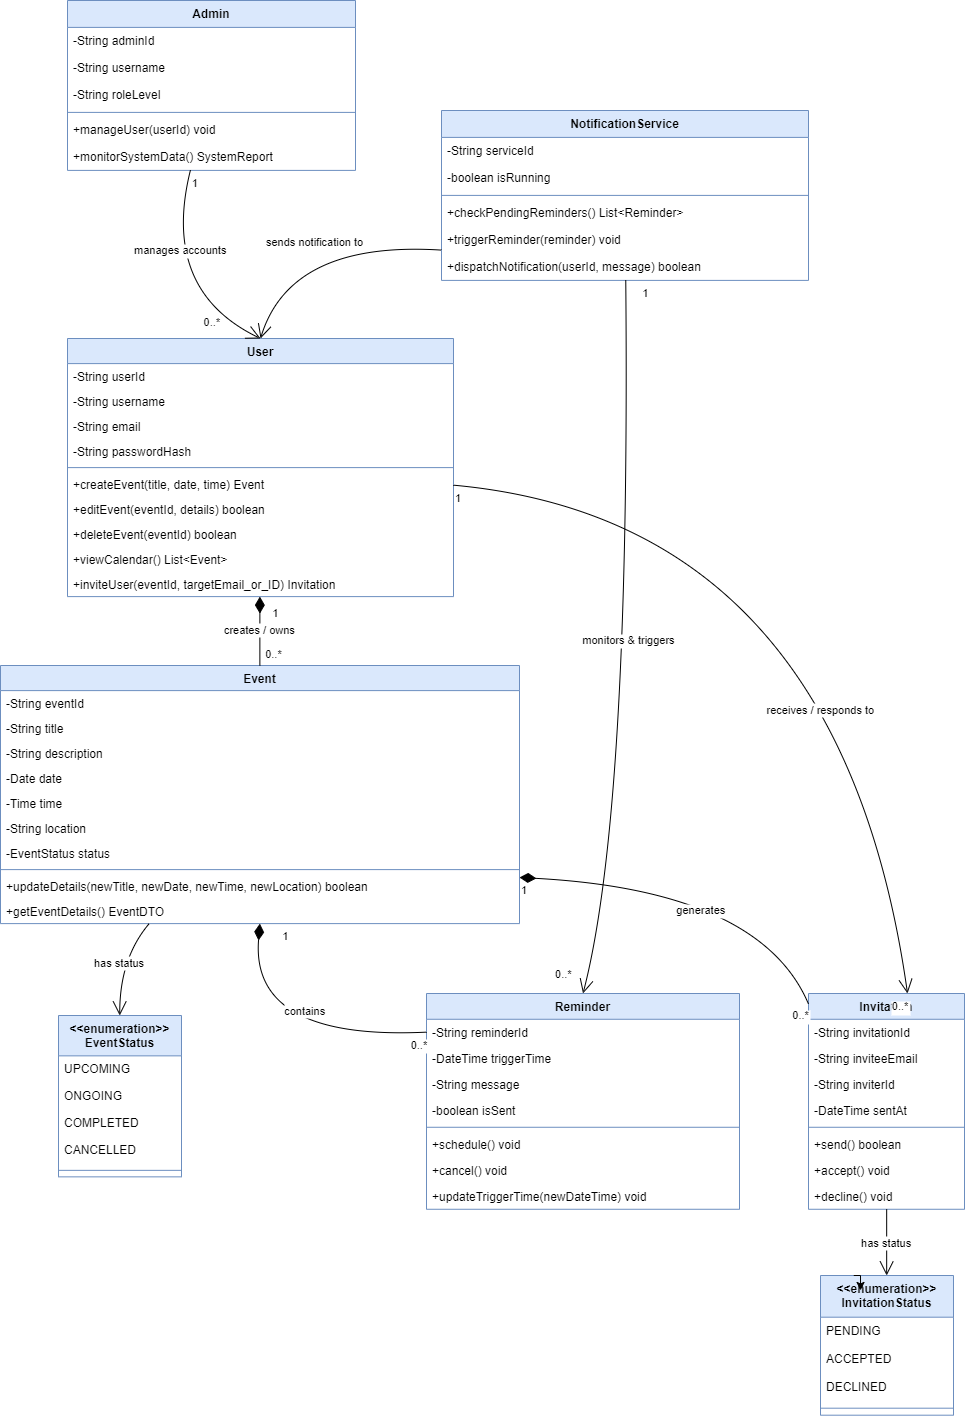
\includegraphics[width=0.85\textwidth]{pictures/classdia.png}
    \caption{Class Diagram mô tả cách hiện thực các trong hệ thống này}
\end{figure}
%Mục 4
\section{Architecture Design}


\begin{figure}[H]
    \centering
    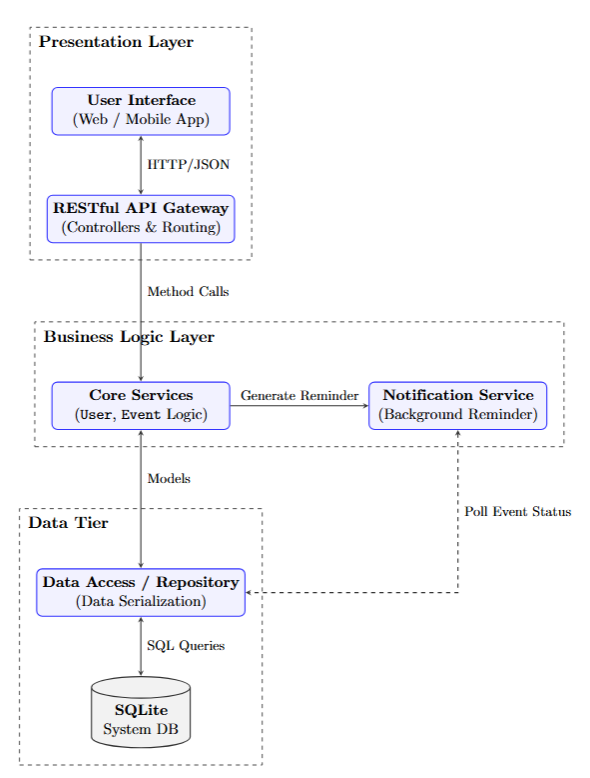
\includegraphics[width=0.75\textwidth]{pictures/archi.png}
    \caption{Sơ đồ Kiến trúc phân tầng của hệ thống SERS}
\end{figure}



\subsection{Các thành phần và Đáp ứng NFR1}
\begin{enumerate}[leftmargin=*]
    \item \textbf{Presentation Layer (Tầng Giao diện):} Nhận thao tác từ người dùng và chuyển tiếp xuống hệ thống (tương ứng với mũi tên "Gửi yêu cầu" trong Hình 1 và 2).
    \item \textbf{Business Logic Layer (Tầng Nghiệp vụ):} Dựa theo Class Diagram (Hình 4), tầng này chứa:
    \begin{itemize}
        \item \textbf{Core Services (\texttt{User}, \texttt{Event}):} Chịu trách nhiệm thực thi các CRUD logic, kiểm tra dữ liệu hợp lệ và chuyển đổi các trạng thái (\texttt{EventStatus}).
        \item \textbf{Notification Service (Đáp ứng NFR1):} Để đảm bảo thông báo gửi trong vòng 60 giây (NFR1), class \texttt{NotificationService} được chạy như một tiến trình ngầm (Background Service). Nó thực thi hàm \texttt{checkPendingReminders()} liên tục truy vấn Data Tier (với chu kỳ quét ngắn khoảng 30s) để \texttt{triggerReminder()} kịp thời.
    \end{itemize}
    \item \textbf{Data Tier (Tầng Dữ liệu):} Lưu trữ toàn bộ thông tin của Hệ thống quản lý SERS, trả kết quả truy vấn ("Xác nhận lưu thành công", "Xác nhận xóa thành công") lên tầng nghiệp vụ.
\end{enumerate}

\subsection{Đề xuất Công nghệ sử dụng}
\begin{itemize}[leftmargin=*]
    \item \textbf{Backend:} \textbf{FastAPI (Python)}. Khung làm việc này nhẹ, hỗ trợ xử lý bất đồng bộ (async), rất phù hợp để hiện thực hóa các class trong Hình 4.
    \item \textbf{Background Task:} \textbf{APScheduler}. Công cụ hoàn hảo để chạy class \texttt{NotificationService} ngầm dưới nền, đáp ứng việc check thời gian liên tục mà không làm chậm các API tạo/sửa sự kiện.
    \item \textbf{Database:} \textbf{SQLite}. Tích hợp sẵn trong Python, đủ mạnh để lưu trữ dữ liệu dự án môn học.
\end{itemize}

%Mục 5
\section{Implementation and Code Quality}
\subsection{Code Listing}
Link source code: \href{https://github.com}{Click here}
\subsection{Short Inspection Summary}

\begin{table}[H]
\centering
\begin{tabularx}{\linewidth}{|l|X|}
\hline
\textbf{Tiêu chí} & \textbf{Mô tả} \\
\hline
Đặt tên rõ ràng & Các lớp (Event, EventManager), hàm (create\_event, delete\_event) và biến (event\_date, reminder\_minutes) được đặt tên có ý nghĩa, thể hiện rõ mục đích sử dụng. \\
\hline
Thụt lề nhất quán & Tuân theo chuẩn PEP 8: thụt lề 4 khoảng trắng; sử dụng dòng trống để phân tách các khối logic. \\
\hline
Chú thích và docstring & Mỗi lớp và các hàm công khai đều có docstring; comment được dùng để giải thích các logic không rõ ràng. \\
\hline
Nguyên lý trách nhiệm đơn & Lớp Event chỉ chứa dữ liệu; EventManager xử lý toàn bộ logic CRUD và kiểm tra dữ liệu. \\
\hline
Kiểm tra đầu vào & Sử dụng các hàm private riêng (\_validate\_title, \_validate\_datetime, \_validate\_reminder) giúp hàm create\_event rõ ràng hơn. \\
\hline
\end{tabularx}
\caption{Đánh giá chất lượng mã nguồn}
\end{table}

\begin{table}[H]
\centering
\begin{tabularx}{\linewidth}{|l|l|X|X|}
\hline
\textbf{ID} & \textbf{Loại vấn đề} & \textbf{Vấn đề phát hiện} & \textbf{Cách khắc phục đề xuất} \\
\hline
I-01 & Naming & Dict \_events dùng tên quá chung (e dict) & Đổi thành \_event\_store hoặc \_event\_registry để rõ nghĩa hơn \\
\hline
I-02 & Missing check & create\_event không dùng strip() cho description trước khi lưu & Thêm description = description.strip() trước khi tạo Event \\
\hline
I-03 & Readability & to\_dict() không bao gồm trường created\_at, không nhất quán với constructor & Thêm 'created\_at': self.created\_at vào dict trả về \\
\hline
I-04 & Missing check & reminder\_minutes không có giới hạn trên; giá trị rất lớn vẫn được chấp nhận & Thêm kiểm tra giới hạn trên (ví dụ: <= 10080 cho tối đa 1 tuần) \\
\hline
I-05 & Documentation & list\_events() thiếu docstring mô tả kiểu trả về & Thêm annotation kiểu trả về List[Event] và bổ sung docstring \\
\hline
\end{tabularx}
\caption{Kết quả peer-review}
\end{table}

\subsection{Code Smells and Refactoring}
\subsubsection{Code Smell 1 - Long Method (create\_event)}
\noindent\textbf{Vấn đề:} \\
Hàm \texttt{create\_event} gọi ba hàm kiểm tra (validation) riêng biệt. Dù mỗi hàm đều nhỏ, nhưng khi hệ thống mở rộng, nhiều kiểm tra khác (ví dụ: kiểm tra sự kiện trùng lặp, kiểm tra định dạng địa điểm) sẽ tiếp tục được thêm trực tiếp vào \texttt{create\_event}, khiến hàm này trở nên dài và khó quản lý.

\vspace{5pt}

\noindent\textbf{Refactoring:} \\
Tách ra một hàm duy nhất \texttt{\_validate\_all(title, date, time, reminder)} để gọi tất cả các hàm kiểm tra con. Khi đó, \texttt{create\_event} chỉ cần gọi \texttt{\_validate\_all(...)} để giữ độ dài hàm dưới 10 dòng. Cách này tuân theo mẫu refactoring \textit{Extract Method}.

\begin{lstlisting}[style=python]
# Before (smell)
def create_event(self, title, date, time, ...):
    self._validate_title(title)
    self._validate_datetime(date, time)
    self._validate_reminder(reminder_minutes)
    # 10+ more lines 

# After (refactored)
def _validate_all(self, title, date, time, reminder):
    self._validate_title(title)
    self._validate_datetime(date, time)
    self._validate_reminder(reminder)

def create_event(self, title, date, time, ...):
    self._validate_all(title, date, time, reminder_minutes)
    new_event = Event(...)
    self._events[new_event.event_id] = new_event
    return new_event
\end{lstlisting}

\subsubsection{Code Smell 2 - Duplicate Logic (get\_event reuse)}
\noindent\textbf{Vấn đề:} \\
Cả \texttt{delete\_event} và các hàm trong tương lai như \texttt{update\_event} đều cần lấy sự kiện theo ID. Nếu logic tìm kiếm (kiểm tra tồn tại key, ném lỗi \texttt{KeyError}) được viết trực tiếp trong từng hàm, nó sẽ bị lặp lại.

\vspace{6pt}

\noindent\textbf{Refactoring:} \\
Hàm \texttt{get\_event} hiện tại đã gom toàn bộ logic này. Cách cải thiện là đảm bảo mọi hàm cần truy cập sự kiện đều gọi \texttt{get\_event(event\_id)} thay vì truy cập trực tiếp \texttt{self.\_events[event\_id]}. Điều này tuân theo nguyên lý \textit{DRY (Don't Repeat Yourself)}.

\begin{lstlisting}[style=python]
# Before (smell) - direct dict access in delete_event
def delete_event(self, event_id):
    if event_id not in self._events:          # duplicated check
        raise KeyError(...)
    del self._events[event_id]

# After (refactored) - reuse get_event
def delete_event(self, event_id):
    event = self.get_event(event_id)          # centralized check
    del self._events[event_id]
    return True
\end{lstlisting}

%Mục 6
\section{Software Testing and Quality Assurance}
\subsection{Các Functions / User Stories Testing}
\begin{itemize}
    \item \textbf{US-1:} Là người dùng, tôi muốn tạo một sự kiện để có thể theo dõi các hoạt động sắp tới.
    \item \textbf{US-2:} Là người dùng, tôi muốn nhận thông báo lỗi khi nhập dữ liệu không hợp lệ để đảm bảo danh sách sự kiện luôn chính xác.
    \item \textbf{US-3:} Là dịch vụ thông báo, tôi muốn các nhắc nhở được kích hoạt đúng thời điểm để người dùng được thông báo đúng lịch.
\end{itemize}
\subsection{Test Plan}
\begin{table}[H]
\centering
\begin{tabularx}{\linewidth}{|l|X|}
\hline
\textbf{Thuộc tính} & \textbf{Chi tiết} \\
\hline
Mục tiêu & Xác minh rằng SERS tạo sự kiện đúng với dữ liệu hợp lệ, từ chối dữ liệu không hợp lệ với thông báo lỗi rõ ràng, và kích hoạt nhắc nhở đúng thời điểm đã lên lịch. \\
\hline
Mức kiểm thử & Unit test cho các phương thức của EventManager; System test cho toàn bộ luồng gửi nhắc nhở. \\
\hline
Phương pháp kiểm thử & Black-box để kiểm tra tính đúng đắn chức năng; White-box (luồng xóa) để xác minh trạng thái nội bộ sau khi thực hiện. \\
\hline
Môi trường kiểm thử & Python 3.11 với framework unittest; sử dụng mock datetime để kiểm tra thời gian nhắc nhở. \\
\hline
Tiêu chí đạt & Tất cả đầu ra mong đợi khớp với kết quả thực tế; không có ngoại lệ chưa được xử lý. \\
\hline
\end{tabularx}
\caption{Kế hoạch kiểm thử hệ thống SERS}
\end{table}
\subsection{Test Cases}

\begin{table}[H]
\centering
\begin{tabularx}{\linewidth}{|l|X|X|X|l|l|}
\hline
\textbf{Test ID} & \textbf{Mô tả} & \textbf{Input} & \textbf{Kết quả mong đợi} & \textbf{Loại test} & \textbf{Mức} \\
\hline

T1 & Tạo sự kiện với dữ liệu hợp lệ &
title="Team Meeting" \newline date="2026-05-10" \newline time="09:00" & 
Trả về đối tượng Event với các trường chính xác; sự kiện được lưu trong manager &
Black-box & Unit \\
\hline

T2 & Tạo sự kiện với tiêu đề rỗng &
title="" \newline date="2026-05-10" \newline time="09:00" &
Phát sinh ValueError: "Event title cannot be empty." &
Black-box & Unit \\
\hline

T3 & Tạo sự kiện với ngày trong quá khứ &
title="Past Event" \newline date="2020-01-01" \newline time="08:00" &
Phát sinh ValueError: "Event must be scheduled in the future." &
Black-box & Unit \\
\hline

T4 & Xóa sự kiện tồn tại &
event\_id hợp lệ từ T1 &
Trả về True; sự kiện không còn trong list\_events() &
White-box & Unit \\
\hline

T5 & Kích hoạt nhắc nhở đúng thời điểm &
event\_time="10:00" \newline now="09:45" \newline reminder=15 min &
Thông báo được kích hoạt chính xác lúc 09:45 &
Black-box & System \\
\hline

\end{tabularx}
\caption{Danh sách test case}
\end{table}


\subsection{ Test Automation Approach}
Các test case ở trên có thể được tự động hóa bằng cách sử dụng framework unittest tích hợp sẵn của Python hoặc pytest. Bên dưới là một ví dụ kiểm thử tự động tiêu biểu cho T1 và T2.

Việc chạy pytest trong quy trình CI/CD (ví dụ: GitHub Actions) sau mỗi lần commit giúp phát hiện sớm các lỗi hồi quy (regression) và tự động ghi lại kết quả kiểm thử. Báo cáo độ bao phủ kiểm thử (test coverage) có thể được tạo bằng pytest-cov để theo dõi những dòng mã đã được thực thi.


%Mục 7
\section{Reflection and Retrospective}

Vào tối thứ Tư ngày 06/05/2026, nhóm tổ chức một buổi họp ngắn để nhìn lại toàn bộ quá trình thực hiện dự án Smart Event Reminder System (SERS). Mục tiêu của buổi họp không chỉ là kiểm tra phần nào đã hoàn thành, mà còn để mỗi thành viên nêu lại góc nhìn của mình về cách nhóm chia việc, phối hợp, xử lý phạm vi và giữ sự nhất quán giữa các phần trong báo cáo. Vì đây là một dự án thiên về quy trình công nghệ phần mềm hơn là xây dựng một sản phẩm hoàn chỉnh, nhóm tập trung đánh giá cách các phần Requirements, Planning, Modeling, Architecture, Implementation và Testing liên kết với nhau. Phần retrospective dưới đây được trình bày theo khung Start / Stop / Continue để rút ra những điểm cần cải thiện cho các dự án sau.

\subsection{Team Retrospective: Start / Stop / Continue}

\begin{table}[H]
\centering
\renewcommand{\arraystretch}{1.5}
\begin{tabularx}{\linewidth}{|l|X|}
\hline
\textbf{Category} & \textbf{Team Reflection} \\
\hline
\textbf{Start} & Nhóm nên bắt đầu thống nhất phạm vi, template trình bày và mối liên hệ giữa các phần ngay từ giai đoạn đầu. Sau mỗi mốc chính, nhóm cũng nên có một bước review ngắn để kiểm tra xem requirements, UML diagrams, architecture, code sample và test cases có đang khớp với nhau hay không. Điều này giúp phát hiện sớm những chỗ lệch trước khi ghép báo cáo cuối cùng. \\
\hline
\textbf{Stop} & Nhóm nên hạn chế việc mỗi thành viên làm phần của mình quá độc lập trong thời gian dài mà không cập nhật tiến độ cho các thành viên khác. Cách làm này có thể khiến nội dung giữa các phần bị lệch, hoặc một thành viên vô tình làm luôn phần việc của người khác. Nhóm cũng nên tránh để việc chỉnh sửa định dạng và kiểm tra tính nhất quán dồn vào cuối deadline. \\
\hline
\textbf{Continue} & Nhóm nên tiếp tục chia công việc theo thế mạnh của từng thành viên và dùng các artefact như backlog, UML diagrams và prototype nhỏ để giữ cho dự án có cấu trúc rõ ràng. Việc chọn phạm vi vừa đủ, chỉ hiện thực một mẫu code minh họa thay vì cố xây dựng toàn bộ hệ thống, là phù hợp với yêu cầu của bài tập. Nhóm cũng nên tiếp tục sử dụng các tài liệu dùng chung để các thành viên dễ theo dõi tiến độ và đóng góp vào báo cáo. \\
\hline
\end{tabularx}
\caption{Tổng kết retrospective của nhóm theo khung Start / Stop / Continue}
\end{table}

\subsection{Lessons Learned}

Qua dự án này, nhóm nhận ra rằng công nghệ phần mềm không bắt đầu từ code mà bắt đầu từ việc hiểu đúng vấn đề, xác định đúng phạm vi và giữ cho các quyết định thiết kế nhất quán với yêu cầu ban đầu. Một user story tốt cần được phản ánh trong acceptance criteria, trong sơ đồ UML, trong kiến trúc hệ thống, trong mẫu hiện thực và cuối cùng là trong test case. Nếu các phần này được viết tách rời, báo cáo có thể vẫn đầy đủ về hình thức nhưng thiếu một dòng chảy kỹ thuật rõ ràng. Scrum và backlog giúp nhóm chia nhỏ công việc, nhưng chỉ thật sự hiệu quả khi task ownership, thời điểm review và tiêu chí hoàn thành được thống nhất rõ. Nhóm cũng học được rằng việc không xây dựng một prototype hoàn chỉnh không phải là thiếu sót trong phạm vi bài này, vì yêu cầu của giảng viên cho phép concept, mock data và pseudo-code. Tuy nhiên, khi chọn hướng minh họa, nhóm vẫn cần trình bày trung thực ranh giới giữa thiết kế đầy đủ trên báo cáo và phần code sample đã hiện thực. Cải tiến quan trọng nhất cho dự án sau không phải là mở rộng phạm vi hệ thống, mà là làm rõ mối liên kết giữa yêu cầu, mô hình, mẫu hiện thực và kiểm thử ngay từ đầu.

\subsection{Individual Reflections}

\begin{table}[h]
\centering
\renewcommand{\arraystretch}{1.5}
\begin{tabularx}{\linewidth}{|l|p{4cm}|X|}
\hline
\textbf{Member} & \textbf{Role} & \textbf{Reflection} \\
\hline
Nguyễn Văn Hùng & Implementation and Code Quality; Software Testing and Quality Assurance & Trong phần hiện thực và kiểm thử, em học được rằng việc tách validation thành các hàm riêng và suy nghĩ kỹ về edge cases ngay từ đầu giúp code dễ bảo trì và ít lỗi hơn. Nếu được làm lại, em sẽ thay các lệnh \texttt{print} bằng logging chuẩn, hiện thực trực tiếp phần code đã refactor thay vì chỉ mô tả, và bổ sung thêm white-box tests để kiểm tra trạng thái nội bộ của hệ thống. \\
\hline
Trần Minh Trí & Process Model and Planning; Architecture Design & Qua phần quy trình Scrum và thiết kế kiến trúc phân tầng, em học được cách lập kế hoạch linh hoạt và cách tách biệt các lớp để hệ thống dễ bảo trì hơn. Nếu có cơ hội làm lại, em sẽ phân tích sâu hơn cơ chế quét của Notification Worker để đảm bảo đáp ứng tốt hơn yêu cầu nhắc nhở trong vòng 60 giây của NFR1. \\
\hline
Nguyễn Tô Quốc Việt & Software Testing and Quality Assurance; Reflection and Retrospective & Trong quá trình tổng hợp retrospective, em nhận ra rằng việc phân chia nhiệm vụ trên bảng phân công là chưa đủ nếu nhóm không cập nhật rõ trạng thái thực hiện của từng phần. Khi phần testing đã được hỗ trợ bởi thành viên khác, em chuyển trọng tâm sang kiểm tra tính nhất quán của toàn bộ báo cáo và rút ra bài học rằng communication sớm quan trọng không kém bản thân việc chia task. \\
\hline
Lê Công Vinh & Requirements Engineering; System Modeling & Qua phần Requirements Engineering và System Modeling, em rèn luyện được kỹ năng tư duy thiết kế phần mềm và đảm bảo sự liên kết từ nhu cầu thực tế của người dùng đến mô hình hệ thống. Nếu được làm lại, em sẽ phân tích sâu hơn các kịch bản ngoại lệ trong State Diagram và Sequence Diagram để cải thiện khả năng xử lý lỗi của hệ thống. \\
\hline
\end{tabularx}
\caption{Phản ánh cá nhân của từng thành viên}
\end{table}




\end{document}
